
\documentclass[preprint,3p,twocolumn]{elsarticle}


\usepackage[x11names,dvipsnames,table]{xcolor} %for use in color links
\usepackage[subrefformat=parens,labelformat=parens]{subfig}
\usepackage{svg}
\usepackage{url}
\usepackage{flushend}
\usepackage{xspace}
\usepackage{enumitem}
\usepackage{hyperref}
\usepackage{multirow}
\usepackage{pbox}

\definecolor{ao(english)}{rgb}{0.0, 0.5, 0.0}
\newcommand{\todo}[1]{\color{blue}\xspace[\emph{#1}]\xspace\color{black}}
\newcommand{\note}[2]{\textbf{\Large{\color{blue}\footnote{{\color{blue}\textbf{#1:} \textit{#2}\color{black}}}}}}
\newcommand{\closednote}[4]{}


\renewcommand\thesubfigure{\Roman{subfigure}}

\journal{Future Generation Computer Systems}

\begin{document}

\begin{frontmatter}

%% Title, authors and addresses

%% use the tnoteref command within \title for footnotes;
%% use the tnotetext command for theassociated footnotes;
%% use the fnref command within \author or \address for footnotes;
%% use the fntext command for theassociated footnote;
%% use the corref command within \author for corresponding author footnotes;
%% use the cortext command for theassociated footnote;
%% use the ead command for the email address,
%% and the form \ead[url] for the home page:
%% \title{Title\tnoteref{label1}}
%% \tnotetext[label1]{}
%% \author{Name\corref{cor1}\fnref{label2}}
%% \ead{email address}
%% \ead[url]{home page}
%% \fntext[label2]{}
%% \cortext[cor1]{}
%% \address{Address\fnref{label3}}
%% \fntext[label3]{}

\title{Software Architectures to Integrate Workflow Engines in Science Gateways}

%% use optional labels to link authors explicitly to addresses:
%% \author[label1,label2]{}
%% \address[label1]{}
%% \address[label2]{}

\author[mcgill,creatis]{Tristan Glatard}
\author[mcgill]{Marc-\'Etienne Rousseau}
\author[creatis]{Sorina Camarasu-Pop}

\author[mcgill]{Reza Adalat}
\author[mcgill]{Natacha Beck}
\author[mcgill]{Najmeh Khalili-Mahani}
\author[criugm]{Pierre-Olivier Quirion}
\author[mcgill]{Pierre Rioux}

\author[criugm]{Pierre Bellec}
\author[mcgill]{Alan C. Evans}

\address[mcgill]{McGill Centre for Integrative Neuroscience, Montreal Neurological Institute, McGill University, Canada.}
\address[creatis]{University of Lyon, CNRS, INSERM, CREATIS, Villeurbanne, France.}
\address[criugm]{Centre de Recherche de l'Institut de G\'eriatrie de Montr\'eal CRIUGM, Montreal, QC, Canada.}

\begin{abstract}
  We investigate software architectures commonly used to integrate workflow engines
  in science gateways. Based on our experience with the development
  and operations of the CBRAIN and VIP science gateways, and our past
  involvement in the SHIWA project, we abstract software components
  and interactions in 6 architectures that we use to classify 18
  systems. We compare these architectures using metrics measuring
  integration effort, robustness, extensibility, scalability and other
  specific features. Results show the pros and cons of the different
  architectures: tight integration and sub-tasking require the least
  amount of integration effort and are also the most robust, most
  architectures perform the same in terms of extensibility, the pool
  model is the most scalable and meta-workflows are only available in
  nested workflows and workflow import. These results provide insights
  for software architects on how to integrate science gateways and
  workflow engines.
\end{abstract}

\begin{keyword}
Workflow engines \sep science gateways \sep software architecture.
\end{keyword}

\end{frontmatter}



%\maketitle

\section{Introduction}

Workflow engines are critical components of the ecosystem of tools and
services offered by science gateways to leverage distributed
infrastructures for the efficient execution of applications through
the web. Several software architectures can be adopted to integrate
workflow engines in science gateways, with important consequences on
the required development effort and on the resulting system. This
paper describes, exemplifies and compares such architectures, based on
system-independent representations of their main components and
interactions.

Our analysis is fed by experience gathered from the development and
sustained operation of the CBRAIN~\cite{SHER-14} and
VIP~\cite{GLAT-13} science gateways for medical image analysis during
the past 7 years. It also builds on the lessons learned from several
science gateway and workflow-related projects, including
SHIWA\footnote{\url{http://www.shiwa-workflow.eu}} and related
initiatives.

The remainder of this Section provides background information and
definitions about workflow engines, science gateways and
infrastructures. In Section~\ref{sec:architectures}, we describe 6
architectures in a consistent framework based on the functional
interactions between the main software components involved. In
Section~\ref{sec:evaluation}, we introduce metrics to measure
integration effort, robustness, extensibility, scalability and other
specific features of the architectures. We use these metrics to
evaluate and compare the 6 architectures. The paper closes on a
discussion and conclusion that highlight architectural recommendations
for science gateway and workflow engine architects.

\subsection{Workflow engines}

In the last decade, the e-Science community has developed workflow
systems to help developers access distributed infrastructures such as
clusters, grids, clouds and web services. These efforts resulted in
tools such as Askalon~\cite{fahringer2005askalon},
Hyperflow~\cite{balis2016hyperflow}, MOTEUR~\cite{GLAT-08i},
Pegasus~\cite{deelman2005pegasus,Deelman201517},
Swift~\cite{zhao2007swift}, Taverna~\cite{oinn2004taverna},
Triana~\cite{taylor2007triana}, VisTrails~\cite{callahan2006managing},
WS-PGRADE~\cite{Kacsuk2012} and others. Such workflow engines usually
describe applications in a high-level language that offers specific
data and control flow constructs, parallelization operators, visual
edition features, links with domain-specific tool repositories,
provenance recording, among other features. An overview of workflow
systems features and capability is available
in~\cite{deelman2009workflows}.
% Descriptions and experiments
%conducted with e-Science workflow engines were published in journals
%such as Future Generation Computer Systems and conference venues such
%as WORKS.

At the same time, toolboxes were emerging in various scientific
domains to facilitate the assembly of software components in
consistent ``pipelines''. In neuroimaging, our primary domain of
interest, tools such as Nipype (Neuroimaging in Python, Pipelines and
Interfaces~\cite{gorgolewski2011nipype}), PSOM (Pipeline System for
Octave and Matlab~\cite{bellec2012pipeline}), SPM (Statistical
Parametric Mapping~\cite{ashburner2011spm}) and FSL (FMRIB Software
Library~\cite{Jenkinson2012782}) provide abstractions and functions to
handle the data and computing flow between processes implemented in a
variety of programming languages. Such tools were interfaced to
computing systems, in particular clusters, to handle high-throughput
task executions. For instance, FSL can launch tasks on SGE through its
fsl\_sub tool, Nipype has execution plugins for S/OGE, Torque,
IPython, ssh and multi-processor servers, and PSOM is interfaced to
Torque, SGE, MOAB, LSF, and HTCondor. Some of these tools also support
advanced features such as provenance tracking (Nipype, PSOM),
redundancy detection across analyses to avoid re-computation (PSOM),
and so on. A wide-array of workflows have been implemented using these
pipelines and are now shared across neuroimaging groups
world-wide. These
domain-specific engines represent a tremendous opportunity for science
gateways to leverage existing tools and applications. They nicely
complement e-Science engines that are more oriented towards the
exploitation of distributed computing infrastructures, in particular
grids and clouds.

For the sake of the analysis conducted in this paper, we define a
\emph{workflow engine} (also abbreviated \emph{engine}) as a piece of
software that submits interdependent computing \emph{tasks} to an
\emph{infrastructure} (local server, cluster, grid or cloud) based on
a workflow description (a.k.a \emph{workflow}) and using input data
that may consist of files, database entries or simple parameter
values. Although simplistic, this definition covers both e-Science and
domain-specific engines. Some workflow engines, usually e-Science
ones, may transfer data across the infrastructure, and others, usually
domain-specific ones, may leave this role to external processes. Workflows
may be expressed in any language, including high-level XML or JSON
dialects such as Scufl or Hyperflow, and low-level scripting languages
such as Bash.

\subsection{Science gateways}

Science gateways are used to share resources in a community and to
provide increased performance and capacity through facilitated access to storage and
computing power. They are often accessible through a web interface
that helps users manage access rights, data transfers, task execution
and authentication on multiple computing and storage
locations. Workflow engines are part of this ecosystem as core
components to implement and execute applications.

% Software properties: integration effort, extensibility, robustness,
% scalability, specific features

Integration between workflow engines and science gateways varies
across systems. Some science gateways may be tailored to a particular
engine that manages critical functions such as task execution, data
transfers and authentication. Other gateways may be more general and
host applications executed by different types of
engines. Extensibility is an important property of the integration, as
new workflows are added frequently, different types and versions of
workflow engines may be integrated over time, and different kinds of
infrastructure can be targeted.

Scalability is also an important concern, since science gateways are
multi-user systems that manage substantial amounts of data and execute
computationally-intensive analyses. To this end, science gateways
may include different instances of the same engine type and implement
some load-balancing policy among them. They may also use advanced
task scheduling policies on the infrastructure, e.g. to ensure fairness
among users~\cite{FERR-14,CPE:CPE3708} or to improve
fault-tolerance~\cite{wilkins2008teragrid,FERR-13}.

Architectures showing reduced system complexity will greatly
facilitate the implementation effort towards robust interactions
which, in turn, have a positive impact on characteristics such as
gateway predictability, transparence, general reliability and results
traceability and reproducibility; characteristics that are also key to
a good user experience. \closednote{Marc-Etienne}{I find that
  something is weak in this last paragraph. Robustness will help with
  transparency, sure, but it seems only a small facet.  Also, the text
  seem to timidly favor architectures with less
  components/interactions without much explanation... Complex systems
  can be robust, but at greater costs...  Here is one: "Architectures
  showing reduced system complexity will greatly facilitate the
  implementation effort towards robust interactions which, in turn,
  have a positive impact on characteristics such as gateway
  predictability, transparence, general reliability and results
  traceability and reproducibility; characteristics that are also key
  to a good user experience."}{Tristan}{Agreed.}

Specific features may also be available in science gateways, such as
data vizualisation and quality control, workflow edition, debugging
instruments, social tools among users, etc.

Various science gateways have been developed, including frameworks
used as building blocks to assemble science gateways. The main
frameworks are Apache Airavata~\cite{marru2011apache}, the Catania
Science Gateway Framework~\cite{Ardizzone2012} and
WS-PGRADE/gUSE~\cite{Kacsuk2012}. Numerous science gateway instances
were built using such frameworks\note{Tristan}{Add references}. Other
gateway instances were also built independently from any framework,
using regular web development tools and libraries to access
distributed systems. CBRAIN and VIP are two such science gateways,
from which we gathered experience about the architectures described in
this paper.

CBRAIN\footnote{\url{http://cbrain.mcgill.ca}}~\cite{SHER-14} is an
open-source\footnote{\url{https://github.com/aces/cbrain}}, web-based collaborative platform addressing the
challenges of data-heavy, computation-intensive neuroimaging
research. It offers transparent web-based access to remote data
sources, distributed computing sites, and an array of processing and
visualization tools, within a secure environment. CBRAIN is deployed
at a wide range of computing sites, including a network of national HPC
centers in Canada, one in Korea, one in Germany, and on numerous local
servers. As February 2016, CBRAIN has served over 420 users across 50
cities in 22 countries and has a national computing allocation of 660 CPU years
per annum.

The Virtual Imaging Platform
(VIP\footnote{\url{http://www.creatis.insa-lyon.fr/vip}})~\cite{GLAT-13}
is a web portal for medical simulation and image data analysis. It
leverages computing and storage resources available in the biomed
Virtual Organization of the European Grid Infrastructure (EGI) to
offer an open service to academic researchers worldwide. VIP
completely masks the infrastructure to enable a transparent user
experience. It uses the MOTEUR workflow engine~\cite{GLAT-13} and the
DIRAC pilot-job framework~\cite{tsaregorodtsev2008dirac} to execute
applications on EGI. Almost 900 users were registered in VIP by
April 2016 and the average CPU consumption between January 2013 and
March 2016 was 35 CPU years per month.

The architectures described hereafter also build on experience with
the SHIWA Simulation Platform~\cite{terstyanszky2014enabling}. The
SHIWA Simulation Platform is a WS-PGRADE/gUSE science gateway that was
developed in the European projects
SHIWA\footnote{\url{http://www.shiwa-workflow.eu}} and
ER-flow\footnote{\url{http://www.erflow.eu}}. It focuses on workflow
interoperability for various disciplines, in particular through the
building of meta-workflows, i.e. workflows that are built out of other
workflows. It implements the so-called Coarse-Grained Interoperability
framework where workflow engines are integrated in the science gateway
as other applications and invoked through a dedicated service. The
Fine-Grained Interoperability framework was also developed in the
SHIWA project, where conversions between workflow languages are
achieved through a common intermediate
representation~\cite{plankensteiner-prodan-etal:2013}. \note{Tristan}{Silvia,
  do you think it is legitimate to refer to SHIWA like this in the
  paper, or should we involve Gabor in the writing?}

\subsection{Infrastructures}

In this paper, infrastructure consists of the computing and storage
resources involved in the workflow execution, as well as the software
services used to access these resources. Infrastructures can be composed of
computing or file servers, databases, clusters, grids or clouds. Some
workflow engines and science gateways may assume specific
characteristics about the infrastructure, such as the presence of a
shared file system between the computing nodes, the availability of a
global task meta-scheduler, the presence of a file catalog, etc. In
the analysis presented below, such specific functions are not
discussed. Instead, we consider the infrastructure as an abstract
system that can execute tasks and store data regardless of the
enabling mechanisms.

\section{Architectures}
\label{sec:architectures}

Architectures to integrate workflow engines in science gateways are
diagrammed in Figure~\ref{fig:architectures} using the graphical
notations shown in Figure~\ref{fig:notations}.  \closednote{Marc-e}{A
  few things bother me a bit with the notation fig., making it harder
  to assimilate 1- The interactions are padded in the middle of other
  stuff (Administrator, Data) 2- The Software component example says
  "Science gateway", should it not be empty?  3- The red arrow to
  explain the use of red; it looks like a very specific type of
  interactions instead of the desired "any interactions or components
  can be red meaning...", especially with 'a' and 'd' which the reader
  does not know the meaning yet.  Maybe a little red arrow and square
  with "Red used when specific to workflow execution"?  I don't have a
  great solution...  Red has special meaning, maybe remove it from the
  other pics (workflow eng, tasks) as it creates lots of visual
  interference when looking for red?  4- Order in text jumps all over
  the fig notations. Explanations are given for, in order: Components,
  workflow engine, interactions, abstract interactions, red color,
  tasks, data (no Administrator?)...  Could re-ordering the fig fix
  this? A figure figure legend could go a long way too (are there some
  in this journal?)  }{Tristan}{Marc-E, is Figure 1 better now?}

Architectures are described from their main software \emph{components}
and \emph{interactions}. Software components include science gateway
and infrastructure in all architectures while workflow service,
workflow pool and agent are involved in some architectures only. The
workflow engine itself is represented by a specific symbol enclosed in a dotted rectangle.

Software interactions among these components are represented with
labeled, plain black arrows.  \emph{Abstract} interactions are
specific types of interactions that may be implemented using different
components and interactions. They are represented with dotted arrows
and labeled with \texttt{*}. An architecture that has an abstract
interaction is an abstract architecture that can be instantiated in
various ways.

Red color is used to represent the components and interactions that
are specific to workflow execution, i.e. that are not involved in any
other process. Tasks refer to computing tasks created by the workflow
engine and executed on the infrastructure. Data represents any type of
file or database involved in workflow execution and stored on the
infrastructure. It does not cover workflow parameters such as strings,
numbers, etc. Administrator refers to a science gateway user with
extended privileges to install applications.

The remainder of this section describes the different types of
interactions involved in the architectures. Architectures are then
detailed and illustrated using examples of real
systems. Table~\ref{table:system-classification} summarizes the
classification of a few systems by architecture.

%http://ieeexplore.ieee.org/stamp/stamp.jsp?tp=&arnumber=4782949

\begin{figure}
\centering
\def\svgwidth{0.7\columnwidth}
\input{figures/notations.pdf_tex}
\caption{Graphical notations}
\label{fig:notations}
\end{figure}

\begin{figure*}
\centering
\hspace*{0.2\columnwidth}
\subfloat[Tight integration]{
\def\svgwidth{0.6\columnwidth}
\input{figures/tight.pdf_tex}
\label{archi:tight}
}
\hfill
\subfloat[Service invocation]{
\def\svgwidth{0.6\columnwidth}
\input{figures/service.pdf_tex}
\label{archi:service}
\hspace*{0.2\columnwidth}
}\\
\hspace*{0.2\columnwidth}
\subfloat[Sub-tasking]{
\def\svgwidth{0.6\columnwidth}
\input{figures/sub-task.pdf_tex}
\label{archi:sub-task}
}
\hfill
\subfloat[Pool]{
\def\svgwidth{0.6\columnwidth}
\input{figures/agent.pdf_tex}
\label{archi:agent}
\hspace*{0.2\columnwidth}
}\\
\subfloat[Nested workflows. Left: abstract model. Right: instantiation with service invocation.]{
\def\svgwidth{0.9\columnwidth}
\input{figures/nested-1.pdf_tex}
\def\svgwidth{0.9\columnwidth}
\input{figures/nested-2.pdf_tex}
\label{archi:nested}
}\\
\subfloat[Workflow import. Left: abstract model. Right: instantiation with service invocation.]{
\def\svgwidth{0.5\columnwidth}
\input{figures/import-1.pdf_tex}
\hfill
\def\svgwidth{0.5\columnwidth}
\input{figures/import-2.pdf_tex}
\label{archi:import}
}
\caption{Architectures}
\label{fig:architectures}
\end{figure*}
\begin{table*}
\centering
\footnotesize
\rowcolors{1}{white}{gray!25}
\begin{tabular}{ll}
  \textbf{Architecture} & \textbf{Systems} \\
  \hline
  Tight & \pbox{1.5\columnwidth}{
          Catania Science Gateway Framework~\cite{Ardizzone2012},
          Distributed application runtime environment (DARE~\cite{maddineni2012distributed}),
          DECIDE~\cite{ardizzone2012decide}$^{c,n}$, LONI Pipeline Environment$^n$~\cite{dinov2009efficient}
          }
  \\
  Service & \pbox{1.5\columnwidth}{
            Apache Airvata~\cite{marru2011apache}, e-BioInfra~\cite{shahand2015data}$^{w,n}$, HubZero with Pegasus~\cite{CPE:CPE3257}, MoSGrid~\cite{krüger2014mosgrid}$^w$, System in~\cite{wu2010accelerating}, Vine Toolkit~\cite{DBLP:journals/scpe/SzejnfeldDKKKKLPTWDNW10}, Virtual Imaging Platform~\cite{GLAT-13}$^n$, WS-PGRADE/gUSE framework~\cite{Kacsuk2012},
            Science gateways in ~\cite{kacsuk2014science}$^w$
            } \\
  Sub-task & CBRAIN and PSOM~\cite{GLAT-16}$^n$, CBRAIN and FSL$^n$\\
  Pool & SHIWA pool~\cite{ROGE-13}\\
  Nested & \pbox{1.5\columnwidth}{SHIWA Simulation Platform (Coarse-Grained Interoperability~\cite{terstyanszky2014enabling})$^w$, HubZero with Pegasus (via hierarchical workflows)~\cite{Deelman201517} \todo{others}
  }\\
  Import & SHIWA Simulation Platform (Fine-Grained Interoperability)~\cite{plankensteiner-prodan-etal:2013}$^w$
\end{tabular}
\caption{Classification of science gateways based on the architecture used to integrate workflow engines. $^c$: based on the Catania Science Gateway Framework. $^w$: based on WS-PGRADE/gUSE. $^n$: used for neuroimaging.}
\label{table:system-classification}
\end{table*}

\subsection{Interactions}

The interactions involved in the architectures are described below and
labeled consistently with the notations used on
Figure~\ref{fig:architectures}.

\begin{enumerate}[leftmargin=0cm,itemindent=0.65cm,label=\texttt{(\alph*)}]

\item Workflow integration: consists in adding a new workflow to the
  system so that users can execute it. It is triggered by an
  administrator of the science gateway and it results in an interface,
  for instance a web form, where users can enter the parameters of the
  workflow to be executed. The interaction has two aspects:
  (\texttt{a$_1$}) the programs used in the workflow are installed on
  the infrastructure, which may require administrative privileges on
  the infrastructure; (\texttt{a$_2$}) the workflow is configured in
  the science gateway so that it becomes available to users. Note that
  integrating a workflow is not the same process as integrating a
  workflow \emph{engine}.
  
\item Task control: operations to manage tasks on the infrastructure,
  including: authentication, submission, monitoring, termination,
  deletion, etc. Controlling tasks requires to deal with the
  heterogeneous batch managers and meta-schedulers that might be
  available on the infrastructure. When the infrastructure is a grid
  or a cloud, it may for instance be achieved using libraries that
  implement standards such as SAGA (Simple API for Grid
  Applications~\cite{goodale2006saga}), DRMAA (Distributed Resource
  Management Application API~\cite{troger2012distributed}), or OCCI
  (Open Cloud Computing Interface~\cite{edmonds2012toward}).
\item Data control: operations to manage data on the infrastructure,
  such as: upload, download, deletion, browsing, replication, caching,
  etc. Data movements can be triggered by the user in the science
  gateway (\texttt{$c_1$}), to upload input data or download processed
  data. They can also be performed by the workflow engine
  (\texttt{$c_2$}), to transfer workflow data (inputs, outputs, or
  intermediate results) across the infrastructure so that tasks can
  use it. The infrastructure might offer various data storage backends
  with heterogeneous interfaces. \closednote{Marc-Etienne}{this -c2- can be also trigerred
    by the user}{Tristan}{No, it can't: this is by definition an interaction between the workflow engine and the infrastructure. It is used to transfer data to/from tasks. I reworded a bit, is it clearer now?} Tools and services such as
  JSAGA~\cite{reynaud2010uniform} or Data Avenue~\cite{hajnal2014data}
  can be used to homogeneize these interfaces.
\item Workflow control: operations to control workflow execution in an
  engine, including: workflow submission, monitoring, termination,
  etc. Workflow control can be coarse-grained (black box) or
  fine-grained (white box). In a coarse-grained model, the various
  tasks created by a workflow execution are masked and the user only
  has a global view of the workflow execution. In a fine-grained
  model, user is exposed to the workflow topology, i.e. to the outputs
  of the individual tasks, their statuses and so on.
\item Sub-task control: operations used by tasks to submit sub-tasks
  on the infrastructure, including: submission, monitoring,
  termination, deletion, etc. Sub-task control is similar to
  interaction \texttt{b}, except that information about the parent
  task, which submitted a sub-task, is usually available and used for
  additional control. For instance, the parent task may wait for all
  its sub-tasks to complete before finishing, and conversely all the
  sub-tasks may be terminated if the parent task is killed.
\item Pool-agent: specific to the pool architecture described in
  Section~\ref{sec:pool}. This is an interaction used when agents
  retrieve work from a central pool. It covers agent registration and
  de-registration to the pool, protocols to send work from the pool to
  the agent, mechanisms to update work status, and so on. A similar
  type of interaction is used in pilot-job
  systems~\cite{turilli2015comprehensive} and other agent-based
  computing models.
\item Workflow conversion: translation from one workflow language to
  another one. This interaction may not be available or implementable
  for every workflow language. It has been developed mostly for
  well-structured and relatively simple workflow language such as between GWorkflowDL
  and Scufl~\cite{OLAB-09}, and between the 4 languages that were involved in the
  SHIWA initiative. In SHIWA, workflow conversion is done through an
  intermediate representation, the Interoperable Workflow Intermediate
  Representation~\cite{plankensteiner-montagnat-etal:2011}, which
  allows to convert among $n$ workflow languages using $2n$
  interactions instead of $n^2$.
\end{enumerate}


\subsection{Tight integration}

See Figure~\subref*{archi:tight}. The workflow engine is tightly
integrated with the science gateway, which means that it is deployed
on the same machine and potentially shares code, libraries and other
software components with the science gateway. For instance, the
workflow engine might be a portlet in a Liferay portal or a controller
in a Ruby on Rails application. The workflow engine and the science
gateway usually share a database where application, users and other
resources are stored\closednote{sorina}{VIP and Moteur also share the
  WorkflowsDB}{Tristan}{Yes, you are right. This is an example where
  such abstract architectures may not completely apply in real
  life. See comment about ``blended'' architectures in the
  discussion. In case of VIP, the sharing of the DB is more an
  implementation detail rather than a strong architectural pattern: we
  could avoid sharing the DB if we wanted.}.  In this model, task and
data control are both initiated from the science gateway. Interactions
\texttt{b} and \texttt{c$_2$} are initiated from the workflow engine
while \texttt{c$_1$} comes from other parts of the science gateway,
for instance a data management interface. As in any other model, the
installation of new workflows in the science gateway (\texttt{a$_2$})
and infrastructure (\texttt{a$_1$}) is done by an administrator, for
security reasons. This is the model adopted in the Catania Science
Gateway Framework~\cite{Ardizzone2012} (see specific documentation on
workflows\footnote{\url{http://bit.ly/1oQrzvQ}}), in the Distributed
application runtime environment (DARE~\cite{maddineni2012distributed})
and in LONI Pipeline Environment~\cite{dinov2009efficient}.
%The Catania Science Gateway Framework would be a good illustration here (workflow engine is a Java portlet), but I can't find a suitable figure about it.
%CIPRES~\cite{miller2010creating} (on which the Neuroscience gateway
%described in~\cite{sivagnanam2015early} is based) % \note{Tristan}{There is no workflow engine in there.}

\subsection{Service invocation}

\begin{figure*}
\centering
\def\svgwidth{1.5\columnwidth}
\input{figures/VIP.pdf_tex}
\caption{Architecture of the Virtual Imaging Platform (service
  invocation).  Step \texttt{3} corresponds to interaction \texttt{d}
  on Figure~\ref{fig:architectures}, step \texttt{2} corresponds to
  interaction \texttt{c$_1$}, and step \texttt{4} maps to interactions
  \texttt{b} and \texttt{c$_2$} (in VIP, workflow data transfers are
  performed by the tasks and embedded in their descriptions).}
\label{fig:vip-architecture}
\end{figure*}

See Figure~\subref*{archi:service}. The workflow engine is available
externally to the science gateway, in a service. The science gateway
controls the service through a specific interaction (\texttt{d}) that
might be implemented as a web-service call (e.g., RESTful or SOAP), as
a command-line or as any other method that offers a well-defined
interface to the workflow engine. The workflow engine might be invoked
either as a black box that completely masks the infrastructure and
tasks, or as a white box that allows for some interaction with
them. The workflow engine is responsible for controlling the tasks on
the infrastructure (\texttt{b}) and for performing the required data
transfers to execute them (\texttt{c$_2$}). User data is usually
managed through the science gateway (\texttt{c$_1$}), although it
might as well be delivered by the workflow engine directly to the
user.

This architecture is largely adopted, in systems such as Apache
Airvata~\cite{marru2011apache}, Vine
Toolkit~\cite{DBLP:journals/scpe/SzejnfeldDKKKKLPTWDNW10}, Virtual
Imaging Platform~\cite{GLAT-13}, the system
in~\cite{wu2010accelerating} and the WS-PGRADE/gUSE
framework~\cite{Kacsuk2012}. The integration between the
HubZero science gateway and the Pegasus workflow engine performed
in~\cite{CPE:CPE3257} also uses a service architecture where the
\texttt{d} interaction is implemented as a set of calls to Pegasus'
command-line tools (e.g., pegasus-status, pegasus-plan,
etc.). Figure~\ref{fig:vip-architecture} shows the architecture of the
Virtual Imaging Platform, where the MOTEUR workflow
engine~\cite{GLAT-08i} is invoked through a service.

\subsection{Sub-tasking}

See Figure~\subref*{archi:sub-task}. The workflow engine is a particular
task that can submit sub-tasks to the science gateway through
interaction \texttt{e}. The workflow engine keeps track of the
dependencies between the sub-tasks, but their execution is delegated to
the science gateway that executes them on the infrastructure through
interaction \texttt{b}. Although the science gateway has no global
vision of the workflow, it can keep track of the sub-tasks submitted
by a given task, for instance to be able to cancel them when the task
is canceled. The science gateway may also implement mechanisms to
facilitate the handling of task dependencies, for instance basic
dependency lists as available in most batch managers (see for instance
attribute \texttt{depend} of option \texttt{-W} in
Torque\footnote{\url{http://docs.adaptivecomputing.com}}).

The science gateway also transfers both user and workflow data across
the infrastructure, so that interactions \texttt{c$_1$} and
\texttt{c$_2$} are both covered by \texttt{c}. In practice, both
\texttt{c$_1$} and \texttt{c$_2$} can be implemented using the same
pieces of code.

The sub-tasking architecture is implemented in CBRAIN~\cite{SHER-14}
where it is used to integrate the FSL toolkit~\cite{Jenkinson2012782}
and the PSOM workflow engine~\cite{bellec2012pipeline}.

The CBRAIN-FSL integration allows to leverage FSL pipelines written in
low-level workflow languages (Linux executables and scripts) that
submit tasks uniformly through a specific tool called fsl\_sub. It is
diagrammed in Figure~\ref{fig:cbrain-fsl-architecture}, where the
science gateway is represented by components \texttt{CBRAIN portal}
and \texttt{CBRAIN execution server} and the infrastructure consists
of \texttt{Storage servers} and \texttt{Computing cluster with shared
  file system}.

The CBRAIN-PSOM integration~\cite{GLAT-16} is shown on
Figure~\ref{fig:cbrain-psom-architecture}. The PSOM workflow engine
adopts a pilot-job architecture~\cite{turilli2015comprehensive} where
a master coordinates workflow execution by submitting workers and
establishing direct communication channels with them. Note how this
peculiar execution model is totally supported by the sub-tasking
architecture.

\begin{figure*}
\centering
\subfloat[CBRAIN-FSL integration.]{
\def\svgwidth{\columnwidth}
\input{figures/CBRAIN-FSL.pdf_tex}
\label{fig:cbrain-fsl-architecture}
} \hfill \subfloat[CBRAIN-PSOM integration. Figure
reproduced from~\cite{GLAT-16}]{ \def\svgwidth{\columnwidth}
  \input{figures/CBRAIN-PSOM.pdf_tex}
\label{fig:cbrain-psom-architecture}
}
\caption{CBRAIN architecture for workflow engine integration
  (sub-tasking).  1: User sends data and workflow execution request to
  storage server(s) and CBRAIN portal. 2: CBRAIN portal sends
  execution request to execution server on cluster. 3: Execution
  server transfers data from storage server(s). 4-5: Execution server
  starts workflow engine (FSL tool or PSOM master) via task
  scheduler. 6: Workflow engine submits sub-tasks to execution server
  (FSL tasks or PSOM agents). 7-8: Execution server starts sub-tasks
  through task scheduler. 8': (PSOM only) PSOM master and workers
  execute workflow. 9. Execution server transfers results to storage
  server(s). Interaction \texttt{b} in Figure~\ref{fig:architectures}
  is implemented by steps \texttt{4}, \texttt{5}, \texttt{7} and
  \texttt{8} (regular interactions with batch manager). Interaction
  \texttt{c} is implemented by steps \texttt{3} and
  \texttt{9}. Interaction \texttt{e} is implemented by step \texttt{6}
  (for FSL: through a modified version of the fsl\_sub script
  available in \url{https://github.com/aces/cbrain-plugins-neuro}; for
  PSOM: through a specific development in PSOM).}
\label{fig:cbrain-sub-tasking}
\end{figure*}

\subsection{Pool model}
\label{sec:pool}
See Figure~\subref*{archi:agent}. Workflows are submitted by the science
gateway to a pool through interaction \texttt{d}. Agents connect to
the pool asynchronously to retrieve and execute workflows through
interaction \texttt{f}. Agents may be started according to various
policies, for instance to ensure load balancing. Agents may wrap
different types of workflow engines. Workflow engine controls tasks
and data on the infrastructure through interactions \texttt{b} and
\texttt{c$_2$}, science gateway transfers user data through
interaction \texttt{c$_1$}, and administrator installs workflows
through interaction \texttt{a$_1$} and \texttt{a$_2$}.

The pool model was implemented in the SHIWA pool~\cite{ROGE-13}
diagrammed in Figure~\ref{fig:shiwa-pool-architecture}. In this
Figure, interaction \texttt{d} of Figure~\subref*{archi:agent} is
implemented in 3 different types of calls to the pool: workflow
submission (\texttt{1} \& \texttt{2}), workflow status retrieval
(\texttt{0} \& \texttt{3})\closednote{sorina}{I suppose letters come here 
from the initial pool-model figure; it's a bit puzzling when mixed with 
letters from Fig 2}{Tristan}{Fixed.}, and workflow retrieval (\texttt{13} \&
\texttt{14}). In Figure~\ref{fig:shiwa-pool-architecture},
interaction \texttt{f} of Figure~\subref*{archi:agent} is implemented
through 2 types of calls: workflow instance retrieval (\texttt{4},
\texttt{5} and \texttt{6}), and workflow instance update (\texttt{11}
and \texttt{12}). Workflow instance retrieval is used by the agents to
fetch work from the pool. Workflow instance update is used by the
agents to update workflow statuses. In the SHIWA pool, agents can wrap
different types of workflow engines to execute workflows expressed
with different languages. Calls \texttt{0}, \texttt{7}, \texttt{8} and
\texttt{9} on Figure~\ref{fig:shiwa-pool-architecture} are used by
workflow engine plugins to declare their supported language and launch
engines, and by workflow engines to report their status to the
agent. These calls are specific to the SHIWA Pool implementation of
the \texttt{agent} component and therefore have no corresponding
representation in Figure~\subref*{archi:agent}.

\begin{figure*}
\centering
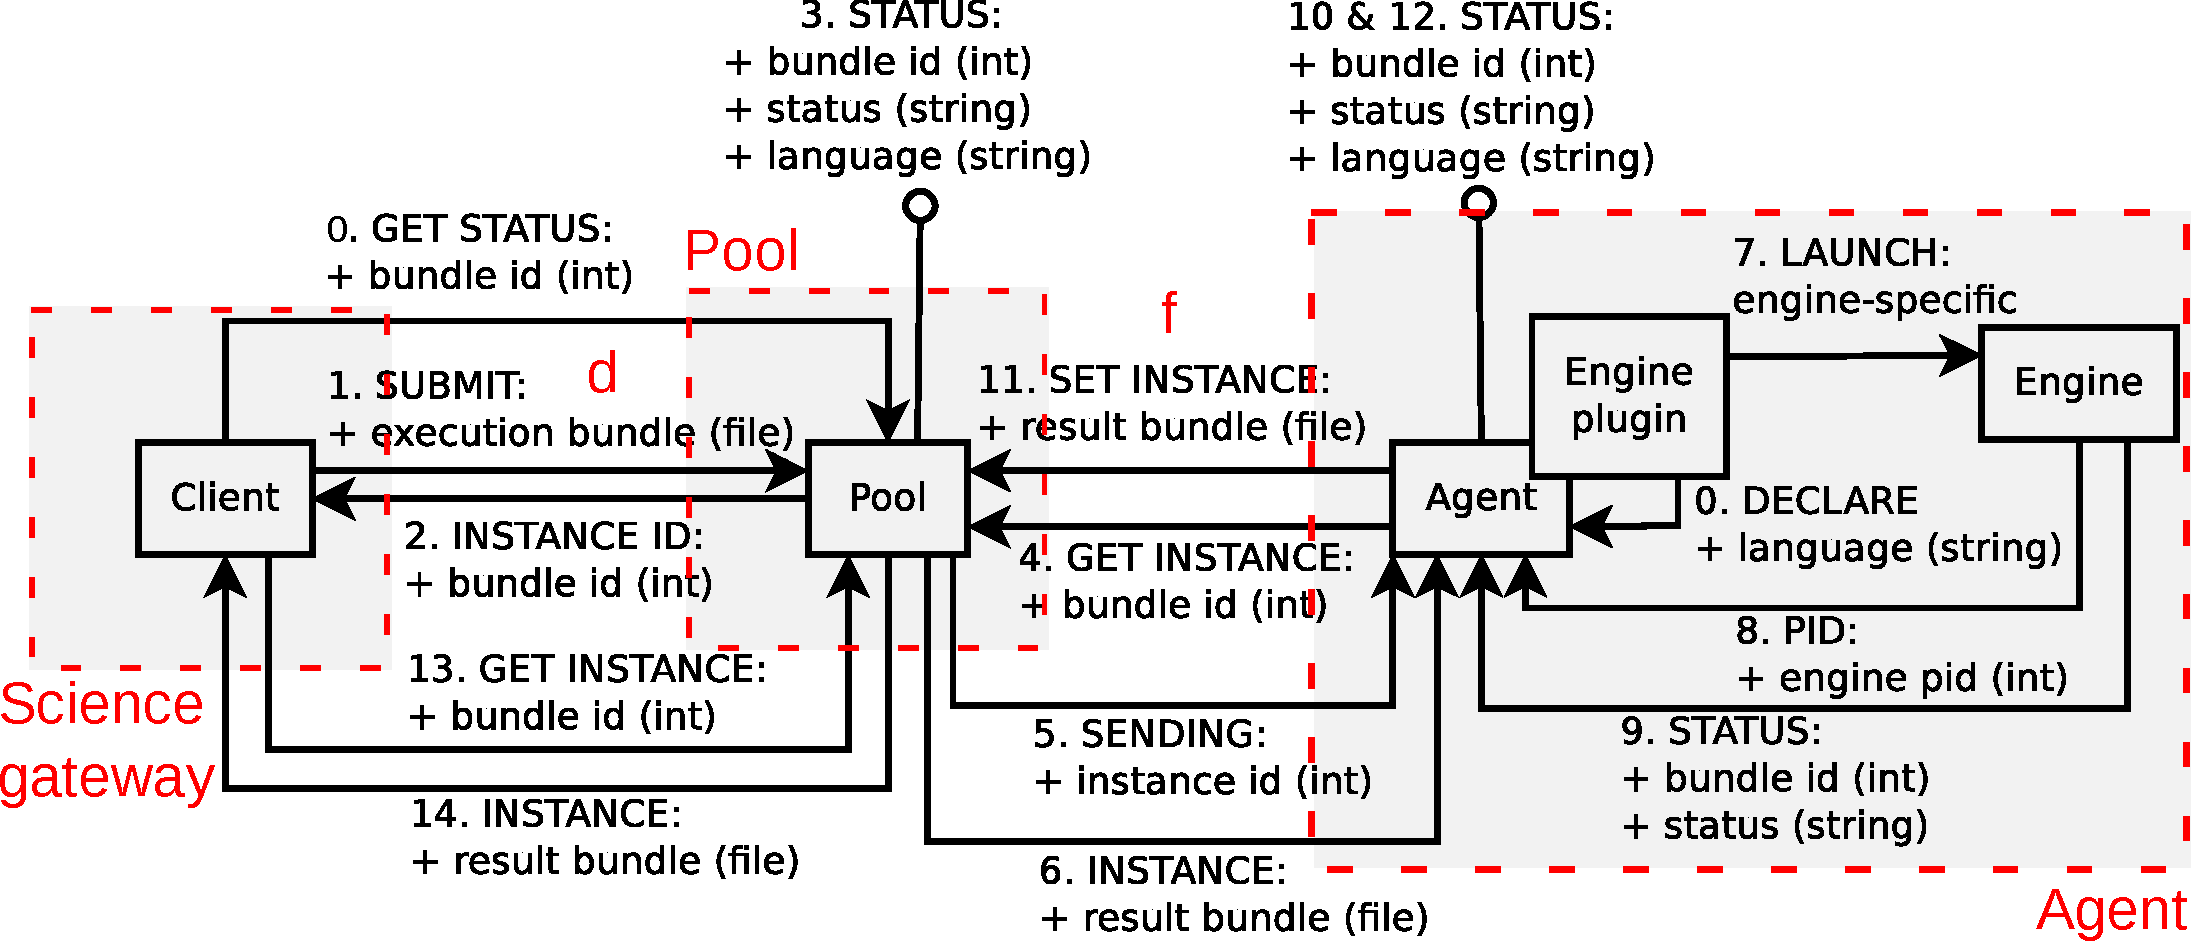
\includegraphics[width=1.5\columnwidth]{figures/pool-interactions.pdf}
\caption{Architecture of the SHIWA pool. Circle-terminated arrows indicate messages
  that are broadcast to all pool clients. Figure reproduced
  from~\cite{ROGE-13}.}
\label{fig:shiwa-pool-architecture}
\end{figure*}


\subsection{Nested workflows}

See Figure~\subref*{archi:nested}. In nested workflows
(Figure~\subref*{archi:nested}-Left), a task of a \emph{parent}
workflow executed by the \emph{parent} engine is itself a workflow,
called \emph{child} workflow, that is executed by a \emph{child}
engine. The parent and child engines might use different workflow
description languages. They might also execute workflows on different
infrastructures. The parent workflow is also called meta-workflow. The
science gateway communicates with the parent engine through abstract
interaction \texttt{*$_1$}. The science gateway also communicates with
the infrastructure to transfer user data through abstract interactions
\texttt{*$_2$} and \texttt{*$_3$}. Both workflow engines communicate
with the infrastructure through abstract interactions \texttt{*$_4$}
and \texttt{*$_5$}. The parent engine communicates with the child
engine through abstract interaction \texttt{*$_6$}. Administrator
installs workflows through interactions \texttt{a$_1$} and
\texttt{a$_2$}.

Nested workflows are abstract architectural patterns that can be
instantiated in the various architectures described previously. We
focus on instantiation with the service invocation model
(Figure~\subref*{archi:nested}-Right) as this is the most used
architecture. In such an instantiation, we assume that the parent and
child workflow engines are distinct pieces of software that require
different workflow services invoked by distinct \texttt{d}
interactions. If this is not the case, then workflow services can be
collapsed in a single one with a \texttt{d} interaction with
itself. An example of such interaction is the use of hierarchical
workflows in Pegasus~\cite{Deelman201517}.
Workflow engines communicate with infrastructures using
\texttt{b} and \texttt{c$_2$}. Science gateway transfers user data to
infrastructures using \texttt{c$_1$} interactions.


Nested workflows have long been available in workflow engines, for
instance in the Taverna workbench~\cite{oinn2004taverna}. They are
also used implicitly in several platforms where workflow engines are
wrapped in workflow tasks as any other command-line tool. Nested
workflows were notably used by the SHIWA Science Gateway to implement
so-called Coarse-Grained workflow
interoperability~\cite{terstyanszky2014enabling}, i.e. to integrate
various workflow engines in a consistent
platform. Figure~\ref{fig:shiwa-architecture} shows the architecture
used in the SHIWA Simulation Platform for nested workflow execution
with service invocation.
\begin{figure*}
\centering
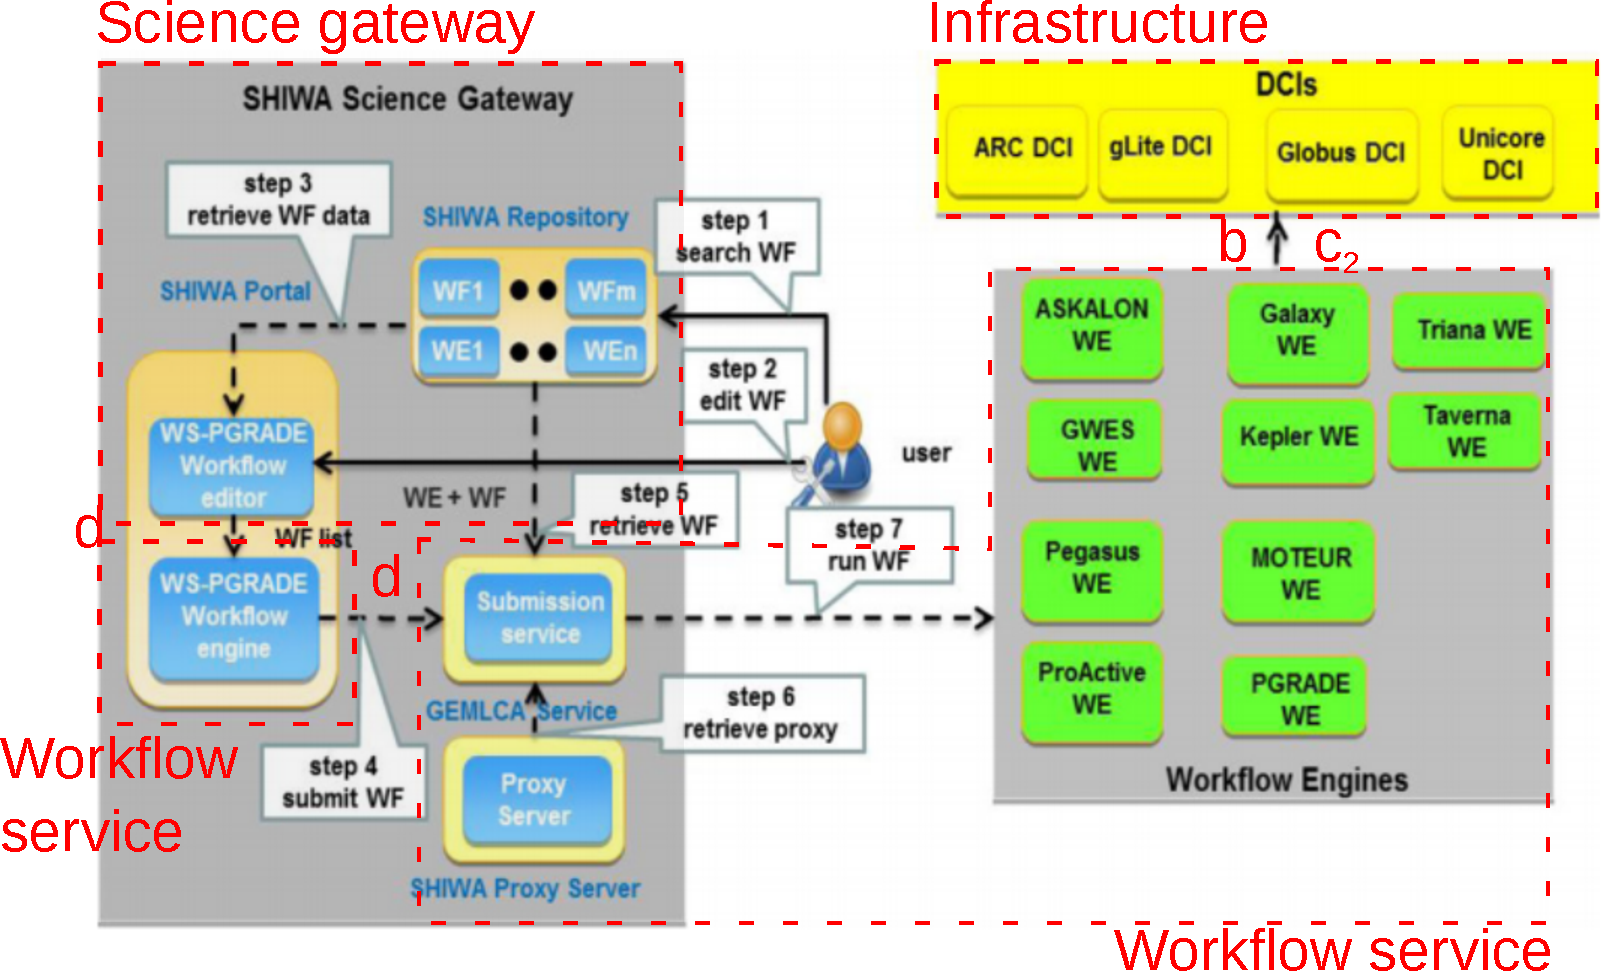
\includegraphics[width=1.5\columnwidth]{figures/shiwa-science-gateway.pdf}
\caption{Nested workflow execution through SHIWA Science Gateway. The
  parent workflow engine is \texttt{WS-PGRADE}, invoked as a service
  in the Science Gateway (step \texttt{1}, interaction \texttt{d} on
  Figure 2(V)-Right. Ten different child engines can be used by nested
  workflows, invoked through the \texttt{Submission service} (step
  \texttt{2}, interaction \texttt{d}). Each of these engines can
  submit tasks and transfer data to a distributed computing
  infrastructure (\texttt{DCI}, step \texttt{3}, interactions
  \texttt{b} and \texttt{c$_2$}). Data interactions (\texttt{c}) and
  application porting ones (\texttt{a}) are not represented. Figure
  reproduced from~\cite{terstyanszky2014enabling} with permission of
  the first author.}
\label{fig:shiwa-architecture}
\end{figure*}

\subsection{Workflow import}

See Figure~\subref*{archi:import}. This is an abstract model 
instantiated with the service invocation architecture for
consistency. Workflows are integrated in the science gateway through
format conversion from a native format to the science gateway
format. Workflow import is usually an offline process which is not
involved in workflow execution. Workflow import was implemented in the SHIWA
Simulation Platform through the IWIR language that provided a common
language for portability across grid workflow
systems~\cite{plankensteiner-prodan-etal:2013}.

\todo{Add description of a real system}

\todo{Refer to ``From the desktop to the grid: scalable bioinformatics via workflow conversion Luis de la GarzaEmail author, Johannes Veit, Andras Szolek, Marc Röttig, Stephan Aiche, Sandra Gesing, Knut Reinert and Oliver Kohlbacher''}

\section{Evaluation}

\label{sec:evaluation}

The architectures described in Section~\ref{sec:architectures} are
evaluated in Table~\ref{table:evaluation}. We use 5 main criteria to
evaluate the architectures: integration effort, robustness of workflow
execution, extensibility, scalability and other specific
features. Criteria break down to specific metrics where \emph{lower
  value indicates better performance}. For each criterion, a total
score is computed by summing up the individual metrics. We ensure that
the different metrics in a criterion measure similar entities so that
they can be summed. The criteria and metrics are explained hereafter.


\begin{table*}
\footnotesize
\centering
\begin{tabular}{rcccccc}
                                     & \textbf{Tight}
                                     & \textbf{Service}
                                     & \textbf{Sub-task}
                                     & \textbf{Pool}
                                     & \textbf{Nested}
                                     & \textbf{Import} \\
\cellcolor[HTML]{EEEEEE}\textbf{Integration effort}& \multicolumn{6}{l}{\cellcolor[HTML]{EEEEEE}}\\
  Total components -- \texttt{I$_1$} & \cellcolor[HTML]{99FF99}2
                                     & \cellcolor[HTML]{99E899}3
                                     & \cellcolor[HTML]{99FF99}2
                                     & \cellcolor[HTML]{99D199}4
                                     & \cellcolor[HTML]{99BB99}5
                                     & \cellcolor[HTML]{99E899}3\\
Total interactions -- \texttt{I$_2$} & \cellcolor[HTML]{99FF99}5
                                     & \cellcolor[HTML]{99F399}6
                                     & \cellcolor[HTML]{99FF99}5
                                     & \cellcolor[HTML]{99E899}7
                                     & \cellcolor[HTML]{99BB99}11
                                     & \cellcolor[HTML]{99E899}7\\
\textbf{Total} (total software pieces) & \cellcolor[HTML]{99FF99}\textbf{7}
                                     & \cellcolor[HTML]{99EF99}\textbf{9}
                                     & \cellcolor[HTML]{99FF99}\textbf{7}
                                     & \cellcolor[HTML]{99E099}\textbf{11}
                                     & \cellcolor[HTML]{99BB99}\textbf{16}
                                     & \cellcolor[HTML]{99E899}\textbf{10}\\
\cellcolor[HTML]{EEEEEE}\textbf{Robustness}& \multicolumn{6}{l}{\cellcolor[HTML]{EEEEEE}}\\
Specific components -- \texttt{R$_1$} & \cellcolor[HTML]{99FF99}0
                                     & \cellcolor[HTML]{99DD99}1
                                     & \cellcolor[HTML]{99FF99}0
                                     & \cellcolor[HTML]{99BB99}2
                                     & \cellcolor[HTML]{99BB99}2
                                     & \cellcolor[HTML]{99DD99}1\\
  Specific interactions -- \texttt{R$_2$} & \cellcolor[HTML]{99F199}2
                                     & \cellcolor[HTML]{99E399}3
                                     & \cellcolor[HTML]{99FF99}1
                                     & \cellcolor[HTML]{99D699}4
                                     & \cellcolor[HTML]{99BB99}6
                                     & \cellcolor[HTML]{99E399}3\\
  \textbf{Total} (execution software pieces)& \cellcolor[HTML]{99F599}\textbf{2}
                                     & \cellcolor[HTML]{99E199}\textbf{4}
                                     & \cellcolor[HTML]{99FF99}\textbf{1}
                                     & \cellcolor[HTML]{99CE99}\textbf{6}
                                     & \cellcolor[HTML]{99BB99}\textbf{8}
                                     & \cellcolor[HTML]{99E199}\textbf{4}\\
\cellcolor[HTML]{EEEEEE}\textbf{Extensibility}& \multicolumn{6}{l}{\cellcolor[HTML]{EEEEEE}}\\
  New engine type -- \texttt{E$_1$}  & \cellcolor[HTML]{99D899}3
                                     & \cellcolor[HTML]{99C499}4
                                     & \cellcolor[HTML]{99EB99}2
                                     & \cellcolor[HTML]{99D899}3
                                     & \cellcolor[HTML]{99BB99}4.5
                                     & \cellcolor[HTML]{99FF99}1\\
New engine version -- \texttt{E$_2$} & \cellcolor[HTML]{99BB99}1
                                     & \cellcolor[HTML]{99FF99}0
                                     & \cellcolor[HTML]{99BB99}1
                                     & \cellcolor[HTML]{99FF99}0
                                     & \cellcolor[HTML]{99FF99}0
                                     & \cellcolor[HTML]{99BB99}1\\
  New workflow -- \texttt{E$_3$} & \cellcolor[HTML]{99FF99}2
                                     & \cellcolor[HTML]{99FF99}2
                                     & \cellcolor[HTML]{99FF99}2
                                     & \cellcolor[HTML]{99FF99}2
                                     & \cellcolor[HTML]{99FF99}2
                                     & \cellcolor[HTML]{99BB99}3\\
New infrastructure -- \texttt{E$_4$} & \cellcolor[HTML]{99E899}3
                                     & \cellcolor[HTML]{99E899}3
                                     & \cellcolor[HTML]{99FF99}2
                                     & \cellcolor[HTML]{99E899}3
                                     & \cellcolor[HTML]{99BB99}5
                                     & \cellcolor[HTML]{99E899}3\\
  \textbf{Total} (difficulty to extend) & \cellcolor[HTML]{99E099}\textbf{9}
                                     & \cellcolor[HTML]{99E099}\textbf{9}
                                     & \cellcolor[HTML]{99FF99}\textbf{7}
                                     & \cellcolor[HTML]{99EF99}\textbf{8}
                                     & \cellcolor[HTML]{99BB99}\textbf{11.5}
                                     & \cellcolor[HTML]{99EF99}\textbf{8}\\
\cellcolor[HTML]{EEEEEE}\textbf{Scalability}& \multicolumn{6}{l}{\cellcolor[HTML]{EEEEEE}}\\
Multiple engine instances -- \texttt{S$_1$}& \cellcolor[HTML]{99BB99}2
                                     & \cellcolor[HTML]{99DD99}1
                                     & \cellcolor[HTML]{99FF99}0
                                     & \cellcolor[HTML]{99FF99}0
                                     & \cellcolor[HTML]{99DD99}1
                                     & \cellcolor[HTML]{99DD99}1\\
Distributed engines -- \texttt{S$_2$}& \cellcolor[HTML]{99BB99}1
                                     & \cellcolor[HTML]{99BB99}1
                                     & \cellcolor[HTML]{99BB99}1
                                     & \cellcolor[HTML]{99BB99}1
                                     & \cellcolor[HTML]{99FF99}0
                                     & \cellcolor[HTML]{99BB99}1\\
Task scheduling -- \texttt{S$_3$}    & \cellcolor[HTML]{99FF99}0
                                     & \cellcolor[HTML]{99FF99}0
                                     & \cellcolor[HTML]{99BB99}1
                                     & \cellcolor[HTML]{99FF99}0
                                     & \cellcolor[HTML]{99BB99}1
                                     & \cellcolor[HTML]{99FF99}0\\
\textbf{Total} (scalability issues)  & \cellcolor[HTML]{99BB99}\textbf{3}
                                     & \cellcolor[HTML]{99DD99}\textbf{2}
                                     & \cellcolor[HTML]{99DD99}\textbf{2}
                                     & \cellcolor[HTML]{99FF99}\textbf{1}
                                     & \cellcolor[HTML]{99DD99}\textbf{2}
                                     & \cellcolor[HTML]{99DD99}\textbf{2}\\
\cellcolor[HTML]{EEEEEE}\textbf{Specific features}& \multicolumn{6}{l}{\cellcolor[HTML]{EEEEEE}}\\
  Meta-workflow  -- \texttt{O$_1$}    & \cellcolor[HTML]{99BB99}1
                                     & \cellcolor[HTML]{99BB99}1
                                     & \cellcolor[HTML]{99BB99}1
                                     & \cellcolor[HTML]{99BB99}1
                                     & \cellcolor[HTML]{99FF99}0
                                     & \cellcolor[HTML]{99FF99}0\\
  Fine-grained debugging -- \texttt{O$_2$}   & \cellcolor[HTML]{99FF99}0
                                     & \cellcolor[HTML]{99FF99}0
                                     & \cellcolor[HTML]{99BB99}1
                                     & \cellcolor[HTML]{99FF99}0
                                     & \cellcolor[HTML]{99BB99}1
                                     & \cellcolor[HTML]{99FF99}0\\
  \textbf{Total} (missing features) & \cellcolor[HTML]{99DD99}\textbf{1}
                                     & \cellcolor[HTML]{99DD99}\textbf{1}
                                     & \cellcolor[HTML]{99BB99}\textbf{2}
                                     & \cellcolor[HTML]{99DD99}\textbf{1}
                                     & \cellcolor[HTML]{99DD99}\textbf{1}
                                     & \cellcolor[HTML]{99FF99}\textbf{0}\\
\end{tabular}

\caption{Architecture evaluation. Lower values (brighter colors) indicate better performance. On each row, metric values are
  normalized between 0 (best value) and 1 (worst value) to determine the
  color of the corresponding table cell. The normalized metric value $m'$ is
  defined as
  $\frac{m-m_{\mathrm{min}}}{m_{\mathrm{min}}-m_{\mathrm{max}}}$ where
  $m$ is the initial metric value, $m_{\mathrm{min}}$ and $m_{\mathrm{max}}$
  are the minimal and maximal values among all architectures. The RGB hexadecimal color code of the cell
  is \texttt{\#99XX99}, where X=F-4m'. \todo{Use 6. Round to the nearest integer.}}
\label{table:evaluation}
\end{table*}

\subsection{Evaluation metrics}

\emph{Integration effort} measures the development required to build
the architecture. It is obtained by counting the total number of
interactions and components on the architecture diagram. It breaks
down to the following 2 metrics:
\begin{itemize}[leftmargin=0cm,itemindent=0.35cm,itemsep=0cm]
\item Total number of components (\texttt{I$_1$}), and
\item Total number of interactions (\texttt{I$_2$}).
\end{itemize}
One may wonder whether infrastructure should be counted in
\texttt{I$_1$} since it is usually not developed by the groups who
integrate workflow engines in science gateway. However, integrating an
infrastructure in the architecture usually requires some technical
effort (e.g., account creation, software installation, etc.), which is
why we keep it in the metric. The two metrics are summed to obtain the
total score for integration effort, which measures the total number of
software pieces to develop (pieces include interactions and
components).

\emph{Robustness of workflow execution} measures the likelihood that
workflow execution fails due to errors in the components or with the
interactions in the software architecture. Note that errors coming
from the infrastructure (e.g., unavailable data or terminated tasks) or
workflows (e.g., wrong user input or application errors) are not
covered since they do not stem directly from the software
architecture. Robustness is determined as the number of software
components and interactions that are specific to workflow execution,
which assumes that complex architectures tend to be prone to failure:
\begin{itemize}[leftmargin=0cm,itemindent=0.35cm,itemsep=0cm]
\item Components (\texttt{R$_1$}): number of specific components
  involved in workflow executions. Science
gateway, for instance, is \emph{not} specific to workflow execution
since it is used to authenticate users, add new workflows, transfer
user data, etc.
\item Interactions (\texttt{R$_2$}): number of specific interactions
  involved in workflow executions.
\end{itemize}
These specific components and interactions are represented in red in
the architecture diagrams in
Figure~\ref{fig:architectures}. \texttt{R$_1$} and \texttt{R$_2$}  are summed to obtain the total score for this
criterion, which measures the total number of software pieces that are
specifically involved in the workflow execution.

\emph{Extensibility} measures the difficulty to replace or add
elements in the architecture. It is determined as the number of
interactions and components that need to be modified when a new
element is added. Modification of a component is required when its
code needs to be updated or recompiled (science gateway or workflow
service), or when a new piece of software has to be installed
(infrastructure only). Modification of an interaction is deemed
necessary when the parameters involved in this interaction are
modified.  Extensibility breaks down in 4 metrics depending on the
type of element that has to be added or replaced:
\begin{itemize}[leftmargin=0cm,itemindent=0.35cm,itemsep=0cm]
\item New engine type (\texttt{E$_1$}): number of interactions or
  components to modify to integrate a new type of workflow engine in
  the architecture. Workflow engines belong to different types when
  they cannot be invoked using the same interface. Adding a new type
  of workflow engine allows to execute more workflows in the science
  gateway.
\item New engine version (\texttt{E$_2$}): number of interactions or
  components to modify to integrate a new version of a workflow engine
  in the architecture, assuming that another version of the same
  engine type is already available. Different versions of a workflow
  engine share the same interface, i.e. they can be invoked using the
  same software. When this is not the case, the different versions are
  considered as different engine types.
\item New workflow (\texttt{E$_3$}): adding a new workflow is a very
  common operation that does not require modifying software components
  or interactions. We measure the difficulty to integrate a new
  workflow by counting the number of interactions required
  to integrate a new workflow in the architecture, assuming
  that the engine type and version required to execute this workflow
  are already available.
\item New infrastructure (\texttt{E$_4$}): number of interactions or components to
  modify to integrate a new type of infrastructure in the
  architecture. Adding a new infrastructure allows to provide more
  computing or storage power, to access specific types of resources
  (e.g., GPUs, clouds), or to enforce execution policies 
  (e.g., constrain data to remain in a particular network domain).\note{Rafael}{Adding a new engine type may also allow run in different infrastructures. Maybe it is worth to put a sentence to clarify that the metric account for it separately.}
%\item New science gateway: \todo{Not sure if this makes sense}.
\end{itemize}
The 4 metrics are summed to obtain a global index that measures the
difficulty to extend the architecture.

\emph{Scalability} corresponds to the ability of the architecture to
cope with high workloads. It is measured by counting the potential
scalability issues in the architectures, i.e. the lack of scalability
features. Features are evaluated using a 3-level metric: 0 means that
the feature is very easy to enable, 1 means that it can be implemented
but with some difficulty, and 2 means that the feature could only be
implemented with a nonsensical amount of effort. Four different
features are identified:
\begin{itemize}[leftmargin=0cm,itemindent=0.35cm,itemsep=0cm]
\item Multiple engine instances (\texttt{S$_1$}): possibility to have
  more than 1 engine instance in the architecture. Workflow engines
  may require important amounts of resources when several workflows,
  or large workflows, are executed. At some point, it may be required
  for the science gateway to distribute the load among several
  engines. \texttt{S$_1$}=0 when adding a new engine instance is a
  fully automated process, i.e. the workflow engine only has to be
  started. In this case, elastic engines are possible, i.e. some kind
  of auto-scaling mechanism can be implemented to control the number
  of engine instances in the architecture. \texttt{S$_1$}=1 when
  adding a new engine instance requires some form of manual
  intervention (e.g., two-factor authentication), which prevents easy 
  implementations of elastic engines. \texttt{S$_1$}=2 when new engine 
  instances cannot be added.
\item Distributed engines (\texttt{S$_2$}): possibility to distribute
  the execution \emph{of a single workflow} among different engine
  instances. In our scope, this feature focuses on the capabilities of
  the architecture rather than these of the workflow
  engine. \texttt{S$_2$}=0 when distributed engines are possible in
  the architecture, and \texttt{S$_2$}=1 when they require specific
  developments in the workflow engine.\note{Rafael}{$S_2$ would be 2 if the paradigm does not allow to distribute the orchestration? e.g., workflow executions implemented within MPI jobs, in Pegasus PMC and dispel4Py.}
\item Task scheduling (\texttt{S$_3$}): task scheduling is a difficult
  issue that depends more on the implementation of specific algorithms
  in the science gateway, workflow engine and infrastructure than on
  the architecture used to integrate the workflow engine in the
  science gateway. Some architectures, however, complexify the task
  scheduling problem by introducing additional software layers or
  create tasks with specific characteristics. \texttt{S$_3$}=0 when
  the architecture does not introduce any additional complexity to the
  scheduling problem, and \texttt{S$_3$}=1 otherwise.
\end{itemize}
The 3 metrics are summed to obtain a global measure of the scalability
issues that are present in the architecture.

\emph{Specific features} include:
\begin{itemize}[leftmargin=0cm,itemindent=0.35cm,itemsep=0cm]
\item Meta-workflow (\texttt{O$_1$}): ability to describe
  meta-workflows from existing workflows. Meta-workflows offer an
  additional level of flexibility to build workflows from reusable
  components. \texttt{O$_1$}=0 when the feature is available,
  \texttt{O$_1$}=1 otherwise.
\item Fine-grained debugging (\texttt{O$_2$}): availability of
  fine-grained debugging information about workflow tasks (white-box
  workflow).  Fine-grained information about workflow tasks is
  required to properly troubleshoot workflow executions.
  \texttt{O$_2$}=0 when such information is easy to access,
  \texttt{O$_2$}=1 otherwise.
\end{itemize}
\texttt{O$_1$} and \texttt{O$_2$} are summed to obtain a total number of missing specific
features in the architecture.

%"A Formal Approach to Support Interoperability in Scientific
%Meta-workflows" (reviewed for IWSG and JoGC) has a formal model to
%evaluate CGI and FGI.
%"four major approaches for workflow interoperability include a,b,c,d" (see Terstyanzky et al, "Enabli%ng scientific workflow sharing through CGI...", FGCS 2014) -> read this ref.
% http://www.oreilly.com/programming/free/files/software-architecture-patterns.pdf

The architectures described in Figure~\ref{fig:architectures} are
evaluated along these metrics in the remainder of this Section.

\subsection{Tight integration}

\paragraph{Integration effort} This architecture does not require any
component in addition to the science gateway and infrastructure
(\texttt{I$_1$=2}). It involves 5 interactions: \texttt{a$_1$},
\texttt{a$_2$}, \texttt{b}, \texttt{c$_1$} and \texttt{c$_2$}
(\texttt{I$_2$=5}).

\paragraph{Robustness} No component is specific to workflow execution
(\texttt{R$_1$}=0), but interactions \texttt{b} and \texttt{c$_2$} are
(\texttt{R$_2$}=2).

\paragraph{Extensibility} Integrating a new type of workflow engine
requires to modify the science gateway as well as interactions
\texttt{b} and \texttt{c$_2$} (\texttt{E$_1$}=3). Updating a workflow
engine version requires modifications in the science gateway
(\texttt{E$_2$}=1).  Inserting a new workflow is done through
interactions \texttt{a$_1$} and \texttt{a$_2$} (\texttt{E$_3$}=2). Adding a new infrastructure generates updates in
interactions \texttt{b}, \texttt{c$_1$} and \texttt{c$_2$}
(\texttt{E$_4$}=3).

\paragraph{Scalability} Adding a new engine instance requires a new
instance of the science gateway, which is in general not possible
(\texttt{S$_1$}=2)\note{Tristan}{What-about load-balancing between web
  server instances?}. Distributed engines are not available by default
(\texttt{S$_2$}=1). The scheduling of tasks on the infrastructure is
as complex as in any other architecture since the workflow engine
might implement any kind of scheduling policy (\texttt{S$_3$}=0).

\paragraph{Specific features} Meta-workflows are not supported by default
(\texttt{O$_1$}=1).  Debugging is not an issue since the science
gateway can retrieve any information from the workflow engine directly
(\texttt{O$_2$}=0).

\subsection{Service invocation}

\paragraph{Integration effort} Service invocation requires a workflow service
in addition to the science gateway and infrastructure
(\texttt{I$_1$}=3). The architecture involves 6 interactions:
\texttt{a$_1$}, \texttt{a$_2$}, \texttt{b}, \texttt{c$_1$},
\texttt{c$_2$} and \texttt{d} (\texttt{I$_2$}=6).

\paragraph{Robustness} The workflow service is a component specific to
workflow execution (\texttt{R$_1$}=1). Workflow execution also
involves 3 specific interactions: \texttt{b},
\texttt{c$_2$} and \texttt{d} (\texttt{R$_2$}=3).

\paragraph{Extensibility} Adding a new type of workflow engine
requires to implement the corresponding workflow service, to modify
interaction \texttt{d}, and to implement interactions \texttt{b} and
\texttt{$c_2$} (\texttt{E$_1$}=4). New engine versions can be added by
updating the workflow service without modifying any interaction or
component (\texttt{E$_2$}=0). We consider that updating the engine
version in a workflow service does not require code updates in the
service since the only goal of this component is to wrap the engine.
New workflows are added in the science gateway or in the workflow
engine through interactions \texttt{a$_1$} and \texttt{a$_2$}
(\texttt{E$_3$}=2). Adding a new type of infrastructure requires
updates in interactions \texttt{b}, \texttt{$c_1$} and \texttt{$c_2$}
(\texttt{E$_4$}=3).

\paragraph{Scalability} The service architecture supports multiple
engine instances through multiple workflow services. In VIP for
instance, this feature has been available from release 1.17 (April
2016). A basic load-balancing mechanism is available that sends new
workflow executions to the engine instance that has the least active
executions. To avoid ``black-hole'' syndromes created by failing
engine instances, engine instances are automatically disabled when
workflows cannot be submitted to them. Adding a new engine instance,
however, requires manual intervention to declare the new instance in
the science gateway (\texttt{S$_1$}=1). Consequently, elastic engines
are difficult to implement because they require a mechanism to update
the science gateway configuration when a new engine instance is
available. Distributing the execution of a single
workflow in multiple engines is usually not possible unless the
workflow engine has specific abilities (\texttt{S$_2$}=1). The
scheduling of tasks on the infrastructure is as complex as in any
other architecture since the workflow engine might implement any kind
of scheduling policy (\texttt{S$_3$}=0).

\paragraph{Specific features} Meta-workflow are not supported by default
(\texttt{O$_1$}=1). Fine-grained debugging information is usually easy
to obtain since the workflow service provides direct access to the
engine (\texttt{O$_2$}=0).

\subsection{Sub-task}

\paragraph{Integration effort} The sub-task architecture requires only 2
components (\texttt{I$_1$}=2).  It involves 5 interactions:
\texttt{a$_1$}, \texttt{a$_2$}, \texttt{b}, \texttt{c} and
\texttt{e} (\texttt{I$_2$}=5).

\paragraph{Robustness} No component is specific to workflow execution
(\texttt{R$_1$}=0), and only interaction \texttt{e} is
(\texttt{R$_2$}=1)\note{sorina}{I understand why this is 1 (and why interactions 
c and b are not counted here), but I wonder whether we can simply ignore these interactions
because they are not specific to workflow execution. As far as robustness is concerned,
the transfers have to be successful anyway...}.

\paragraph{Extensibility} Integrating a new type of workflow engine
requires to develop interaction \texttt{e} and to install the engine
on the infrastructure (\texttt{E$_1$}=2). Updating an engine version
requires updates only on the infrastructure (\texttt{E$_2$}=1).  New
workflows are integrated by creating a new task in the science gateway
through interactions \texttt{a$_1$} and \texttt{a$_2$}  (\texttt{E$_3$}=2). Adding a new
infrastructure requires to update interactions \texttt{b} and
\texttt{c} in the science gateway (\texttt{E$_4$}=2).

\paragraph{Specific features} Meta-workflows are not available
(\texttt{O$_1$}=1).  Obtaining fine-grained information about workflow
tasks is not straightforward since the science gateway has no
knowledge about the workflow topology, and the workflow engine is
integrated as a task (\texttt{O$_2$}=1).

%\todo{Integrating a workflow engine as a sub-task
%only requires to implement interaction \texttt{e} (\texttt{I$_2$}=1)
%and to install the workflow engine on the infrastructure
%(\texttt{I$_3$}=1). A new task type is created in the science gateway
%only when a new workflow has to be integrated (see M$_4$), but this is
%not required to integrate the engine itself (\texttt{I$_1$}=0).}


\paragraph{Scalability}
New engine instances are spawned and executed on the infrastructure as
any other task upon user submission (\texttt{S$_1$}=0). This is a
major interest of the sub-task architecture. Distributed engines are
not supported by default (\texttt{S$_2$}=1). Task scheduling is
slightly more complex than in the other approaches due to the special
role of the task that executes the workflow engine
(\texttt{S$_3$}=1). Indeed, the reliability of this task is critical
since all the sub-tasks in the workflow depend on it and, depending on
the recovery capabilities of the workflow engine, may need to be
resubmitted if the workflow task fails. The workflow task is also
longer than all its sub-tasks, which increases its chances of
failure. In addition, task parameters, for instance estimated
walltime, are more difficult to estimate for the workflow task than
for sub-tasks which may generate issues such as selection of wrong
batch queues on clusters. Finally, the interdependencies between the
workflow task and its sub-tasks may create deadlocks when there is
contention. For instance, if only 1 computing resource is
available for the science gateway and that the workflow task is
running on it and submits sub-tasks, then the sub-tasks could only
execute when the resource is available, which will never happen
because the workflow task will not complete until the sub-tasks
complete. This configuration can be generalized to an infrastructure
with $n$ resources where $n$ workflows are submitted. In practice,
however, the number of submitted workflows usually remains lower than
the number of computing resources available on this infrastructure,
which makes such deadlocks unlikely to happen.

\subsection{Pool}

\paragraph{Integration effort} The pool model requires a workflow pool and an
agent in addition to the science gateway and infrastructure
(\texttt{I$_1$=4}). It involves 7 interactions: \texttt{a$_1$},
\texttt{a$_2$}, \texttt{b}, \texttt{c$_1$}, \texttt{c$_2$}, \texttt{d}
and \texttt{f} (\texttt{I$_2$}=7).

\paragraph{Robustness} The workflow pool and agent are specific to
workflow execution (\texttt{R$_1$=2}). Interactions \texttt{b},
\texttt{c$_2$}, \texttt{d} and \texttt{f} also are (\texttt{R$_2$=4}).

\paragraph{Extensibility} Adding a new engine type requires to wrap
the engine in the agent and to update interactions \texttt{b} and
\texttt{c$_2$} (\texttt{E$_1$=3}). Updating the version of an engine
is transparent (\texttt{E$_2$=0}) since it only requires updating the
agent that is a component dedicated to the engine. Integrating a new workflow is
done through interactions \texttt{a$_1$} and \texttt{a$_2$}
(\texttt{E$_3$=2}). Integrating a new infrastructure requires updates
in interactions \texttt{b}, \texttt{c$_1$} and \texttt{c$_2$}
(\texttt{E$_4$=3}).

\paragraph{Scalability} New engine instances only require new agents,
which is easily automated (\texttt{S$_1$=0}) and by design very
suitable for elastic computing. For instance, auto-scaling rules can
be implemented to start new agents when the workload in the science
gateway exceeds a certain threshold~\cite{lorido2012auto}. Distributed
engines are not available by default (\texttt{S$_2$=1}) and task
scheduling is as complex as in any other architecture
(\texttt{S$_3$=0}).

\paragraph{Specific features} Meta-workflows are not available by default
(\texttt{O$_1$=1}).  Accessing debugging information is not likely to
be an issue since the workflow pool could implement specific functions
for that (\texttt{O$_2$=0}).

\subsection{Nested workflows with service invocation}

\paragraph{Integration effort} Setting up a nested workflow architecture with
service invocation requires a science gateway, 2 workflow services and
2 infrastructures (\texttt{I$_1$=5}). The architecture involves 11
interactions (\texttt{I$_2$=11}): \texttt{a$_1$} (appears twice: once for each
infrastructure), \texttt{a$_2$}, \texttt{b} (twice: once for each
infrastructure), \texttt{c$_1$} (twice: once for each infrastructure),
\texttt{c$_2$} (twice: once for each workflow engine and
infrastructure) and \texttt{d} (twice: once for each workflow engine).

\paragraph{Robustness} The two workflow services are specific to
workflow execution (\texttt{R$_1$=2}). Interactions \texttt{b}
(counted twice), \texttt{c$_2$} (twice) and \texttt{d} (twice) also
are (\texttt{R$_2$=6}).

\paragraph{Extensibility} Adding a new type of \emph{parent} engine
requires to implement the corresponding service, to implement
interactions \texttt{b} and \texttt{c$_2$} in the parent engine, and
to implement interaction \texttt{d} in the science gateway and in the
parent service (\texttt{E$_1$=5}). Adding a new type of \emph{child}
engine only requires to implement the corresponding service, to
develop interactions \texttt{b} and \texttt{c$_2$} in the child
engine, and to implement interaction \texttt{d} in the parent service
(\texttt{E$_1$=4}). We use \texttt{E$_1$=4.5} in
Table~\ref{table:evaluation} to reflect both conditions. Adding a new
version in the parent or child engine only requires modifying this
engine (\texttt{E$_2$=0}). Adding a new
workflow is done through interaction \texttt{a$_1$} and \texttt{a$_2$}
(\texttt{E$_3$=2}). Adding a new infrastructure requires to
re-implement interactions \texttt{b} and \texttt{c$_2$} twice, and
interaction \texttt{c$_1$} once (\texttt{E$_4$=5}).

\paragraph{Scalability} As in the service architecture, adding a new
workflow instance requires manual configuration in the science gateway
(instance of a parent engine), or in the parent engine (instance of a
child engine) (\texttt{S$_1$=1}). Similarly, elastic engines are
difficult to achieve. Distributed engines are
possible, through meta-workflows (\texttt{S$_2$=0}). Task scheduling
is more complex than in other architectures though, due to the fact
that workflow execution is split in different engines (\texttt{S$_3$=1}).

\paragraph{Specific features}
Meta-workflows are possible, which is one of the main interest of this
architecture (\texttt{O$_1$=0}).  Debugging is difficult because the
science gateway cannot directly access fine-grained information in the
sub-workflow (\texttt{O$_2$=1}).

\subsection{Workflow import with service invocation}

\paragraph{Integration effort} Workflow import with service invocation
requires the same components as for service invocation
(\texttt{I$_1$}=3). It requires an additional \texttt{g} interaction
for workflow import (\texttt{I$_1$}=7).

\paragraph{Robustness} Since workflow conversion is not involved in
the execution (it is an offline process), metrics are as in the
service architecture (\texttt{R$_1$=1}, \texttt{R$_2$=3}).

\paragraph{Extensibility} Since adding a new type of workflow engine
aims at supporting more workflows, we consider that it only requires
to re-implement interaction \texttt{g} in this architecture  (\texttt{E$_1$=1}). Note,
however, that implementing interaction \texttt{g} can require very
substantial work depending on the complexity of the language used by
the new engine. Based on the same logic, adding a
new engine version only requires modifying interaction \texttt{g}
(\texttt{E$_2$=1}).  Adding a new workflow is done through
interactions \texttt{a$_1$}, \texttt{a$_2$} and \texttt{g} (\texttt{E$_3$=3}). As in the
service architecture, interfacing with a new infrastructure requires
modifications in the workflow service and in interactions \texttt{b}
and \texttt{c$_2$} (\texttt{E$_4$=3}).

\paragraph{Scalability}  Since workflow conversion is not involved in
the execution (it is an offline process), metrics are as in the
service architecture (\texttt{S$_1$=1},
\texttt{S$_2$=1}, \texttt{S$_3$=0}).

\paragraph{Specific features} Meta-workflows are available after import,
by connecting workflows in the language used in the science gateway
(\texttt{O$_1$=0}). Debugging information is accessible as in the
service invocation architecture (\texttt{O$_2$=0}).

\section{Discussion}

\subsection{Comparison between architectures}

Tight integration and sub-tasking require the least amount of
integration effort, followed by service integration, workflow import
(with service invocation) and pool. Nested workflows (with service
invocation) requires more integration than the other
architectures. Robustness roughly leads to the same ordering of
architectures, with tight integration and sub-tasking in the top
group, service integration and workflow import (with service
invocation) close behind, pool in a third group, and nested workflows
(with service invocation) at the end. This ordering is consistent
across metrics, it reflects the global complexity of the
architectures.

Regarding extensibility, most architectures are overall comparable,
except nested workflows (with service invocation) which is
significantly behind. This is explained by the complexity of the
nested workflow architecture, with 2 infrastructures and 2 workflow
services. Sub-tasking and workflow import (with service invocation)
perform a bit better when integrating new engines (\texttt{E$_1$}), which
is interesting given the current profusion of engines with different
characteristics.  However, sub-tasking, workflow import (with service
invocation) and tight integration perform worse than the others when adding
engine versions (\texttt{E$_2$}) due to the need to update
infrastructure (sub-tasking), science gateway (tight integration), or
workflow converter (workflow import). Workflow import performs worse
than the others when integrating new workflows (\texttt{E$_3$}) because of
the language conversion step. All architectures except nested
workflows perform the same when integrating new infrastructures (\texttt{E$_4$}).

The pool architecture is overall the most scalable, which is not a
surprise since it was designed precisely for scalability. Tight
integration is the least scalable and all the other architectures
perform the same. The overall scalability score, however, should not
mask the unique characteristics of architectures regarding this
criterion. Nested workflows are the only architecture that can easily
accommodate distributed workflow execution, which can be critical in
some cases. At the same time, the scheduling constraints created by
the sub-tasking and nested workflow architectures could well become
showstoppers depending on the type of the targeted
infrastructure. Non-reliable infrastructures, for example, could
hardly cope with workflow engines being wrapped in computing tasks as
done in sub-tasking. The availability of multiple engine instances
could also become a critical feature for science gateways with
important workloads, which would favor sub-tasking and pool.

Differences in other specific features should not be neglected. Nested
workflows (with service invocation) and workflow import (with service
invocation) are the only architectures that support meta-workflows,
which may be interesting in some cases. The availability of
fine-grained debugging information may also be critical to efficient
user support.

Table~\ref{table:overall} provides an overall comparison between
architectures, based on the metrics in Table~\ref{table:evaluation}.
Overall, sub-tasking, and workflow import (with service invocation)
perform a bit better than tight integration, service invocation and
pool. Nested workflows stands a bit behind for the reasons mentioned
previously.
\begin{table*}
\centering
\begin{tabular}{rcccccc}
                                    & \textbf{Tight}
                                    & \textbf{Service}
                                    & \textbf{Sub-task}
                                    & \textbf{Pool}
                                    & \textbf{Nested}
                                    & \textbf{Import} \\
  Integration effort (normalized total) &
                                    \cellcolor[HTML]{99FF99}{0.00}
                                    & \cellcolor[HTML]{99EF99}{0.22}
                                    & \cellcolor[HTML]{99FF99}{0.00}
                                    & \cellcolor[HTML]{99E099}{0.44}
                                    & \cellcolor[HTML]{99BB99}{1.00}
                                      & \cellcolor[HTML]{99E899}{0.33}\\
Robustness (normalized total) &
                                \cellcolor[HTML]{99F599}{0.14}
                                    & \cellcolor[HTML]{99E199}{0.43}
                                    & \cellcolor[HTML]{99FF99}{0.00}
                                    & \cellcolor[HTML]{99CE99}{0.71}
                                    & \cellcolor[HTML]{99BB99}{1.00}
                                    & \cellcolor[HTML]{99E199}{0.43}\\
  Extensibility (normalized total)  & \cellcolor[HTML]{99E099}{0.44}
                                     & \cellcolor[HTML]{99E099}{0.44}
                                     & \cellcolor[HTML]{99FF99}{0.00}
                                     & \cellcolor[HTML]{99EF99}{0.22}
                                     & \cellcolor[HTML]{99BB99}{1.00}
                                     & \cellcolor[HTML]{99EF99}{0.22}\\
Scalability (normalized total)  & \cellcolor[HTML]{99BB99}{1.00}
                                     & \cellcolor[HTML]{99DD99}{0.50}
                                     & \cellcolor[HTML]{99DD99}{0.50}
                                     & \cellcolor[HTML]{99FF99}{0.00}
                                     & \cellcolor[HTML]{99DD99}{0.50}
                                     & \cellcolor[HTML]{99DD99}{0.50}\\
Specific features (normalized total) & \cellcolor[HTML]{99DD99}{0.50}
                                     & \cellcolor[HTML]{99DD99}{0.50}
                                     & \cellcolor[HTML]{99BB99}{1.00}
                                     & \cellcolor[HTML]{99DD99}{0.50}
                                     & \cellcolor[HTML]{99DD99}{0.50}
                                     & \cellcolor[HTML]{99FF99}{0.00}\\
                                    & \cellcolor[HTML]{99EE99}\textbf{2.1}
                                    & \cellcolor[HTML]{99EE99}\textbf{2.1}
                                    & \cellcolor[HTML]{99FF99}\textbf{1.5}
                                    & \cellcolor[HTML]{99F499}\textbf{1.9}
                                    & \cellcolor[HTML]{99BB99}\textbf{4.0}
                                    & \cellcolor[HTML]{99FF99}\textbf{1.5}\\
\end{tabular}
\caption{Overall evaluation. Brighter colors and lower scores indicate better performance. Scores
  are obtained by summing the normalized total scores ($m'$ values) of
  each criterion in Table~\ref{table:evaluation} and the colors are obtained by normalizing these scores
  as done in Table~\ref{table:evaluation}. }
\label{table:overall}
\end{table*}

\subsection{Limitations}

A few limitations remain that should be considered when using the
results of our evaluation. First of all, the evaluation is done at a
quite high-level of abstraction that may be a bit artificial when
applied to real systems. Abstracting architectures from their
implementation in specific systems is useful to compare them, but we
also realize that this comes at the cost of realism.  In particular,
the presented architectures are pure patterns that may be blended in
actual systems. The distinction between tight integration and service
invocation, for instance, may not be that clear in practice. Service
invocation may also be combined with sub-tasking in some cases.

Moreover, all the interactions involved in the architectures were
treated equally, as if they all required similar amounts of
development effort, which is realistically not the case. For example,
interaction \texttt{g} (workflow language conversion) clearly requires
more effort than interaction \texttt{d} (service invocation), and may
create much more reliability issues as well. However, quantifying the
robustness and amount of development associated with each interaction
and software component cannot realistically be done without entering
into the details of a particular system.

The particular case of interaction \texttt{g} (workflow language
conversion) should be further discussed since it is very likely that
this interaction could not be easily generalized to any workflow
language. For instance, converting FSL, PSOM or Nipype pipelines to
any other workflow language is very tricky because these engines rely
on general-purpose programming languages such as Bash, Octave and
Python, which are much richer than scientific workflow languages.

The abstract nested workflows and workflow import patterns were
instantiated with service invocation so that they can be analyzed in
the same framework as the other architectures. Other types of
instantiation, for instance nested workflows with sub-tasking, could
also be envisaged. We chose to limit ourselves to instantiations with
service invocation because the resulting architectures are implemented
in real systems, and because service invocation is largely
used. Nested workflows with sub-tasking, in particular, could be an
interesting architecture to explore.

Finally, the particular technical or historical context of a science
gateway project may obviously influence the choice of an architecture
to integrate workflow engines. For instance, some workflow engines may
be already available as web services, which would tend to favor
service invocation, and other science gateways may have strongly
tested task and data control features (interactions \texttt{b} and
\texttt{c}), which would favor sub-tasking. The migration cost between
architectures is totally ignored as well.

\section{Conclusion}

% Summary of contributions
We reviewed architectures used to integrate workflow engines in
science gateways, we described them in a system-independent framework
suitable for comparison, we illustrated them on real systems, we
developed quantitative metrics for evaluation, we evaluated these
metrics for all the architectures, and we discussed the pros and cons
of all the architectures based on these metrics.

% Impact of the work
To the best of our knowledge, our work is the first of its kind
\note{Tristan}{Be more accurate}. Our results can be used as
recommendation for science gateway and workflow engine architects to
build new platforms, or to upgrade existing ones.

\section{Acknowledgments}

We warmly thank Rafael Ferreira da Silva for its contribution to the
VIP platform and for creating Figure~\ref{fig:vip-architecture}. This
work is in the scope of the LABEX PRIMES (ANR-11- LABX-0063) of
Universit\'e de Lyon, within the program ``Investissements d’Avenir''
(ANR-11-IDEX-0007) operated by the French National Research Agency
(ANR). This work has been made possible with the support of the Irving
Ludmer Family Foundation and the Ludmer Centre for Neuroinformatics
and Mental Health.

\section*{References}

\bibliographystyle{elsarticle-num}
\bibliography{biblio}

\end{document}
\endinput
